\section{La méthode PPanGGOLiN}

Pour construire un graphe de pangénome partitionné, PPanGGOLiN suit une liste d'étapes présentées sur la \autoref{fig:ppanggolin}. En données d'entrée, PPanGGOLiN prend un ensemble de génomes annotés\footnote{Il est conseillé d'utiliser au moins 15 génomes ayant des variations de contenue en gènes pour partitionner correctement le graphe de pangénome.}. Les gènes des génomes seront clusterisés\footnote{Rappel : nous utilisons le mot cluster pour parler du regroupement des gènes en familles par similarité et partitionnement pour l'assignation des familles à une partie dans le pangénome (\textit{core}, \textit{shell}, \textit{cloud}\dots)} en familles de gènes homologues. Ces familles seront utilisées comme n\oe uds pour construire le graphe de pangénome et la relation de voisinage entre les gènes des familles dans les génomes comme arêtes. À partir du graphe de pangénome et de la matrice de présence/absence des familles dans les génomes, PPanGGOLiN applique des algorithmes statistiques et de machine learning pour déterminer le nombre de partitions et assigner les familles à une partie (\textit{persistent}, \textit{shell} ou \textit{cloud}). Le partitionnement est reporté sur le graphe de pangénome pour obtenir le graphe de pangénome partitionné.

\begin{figure}[htbp]
    \centering
    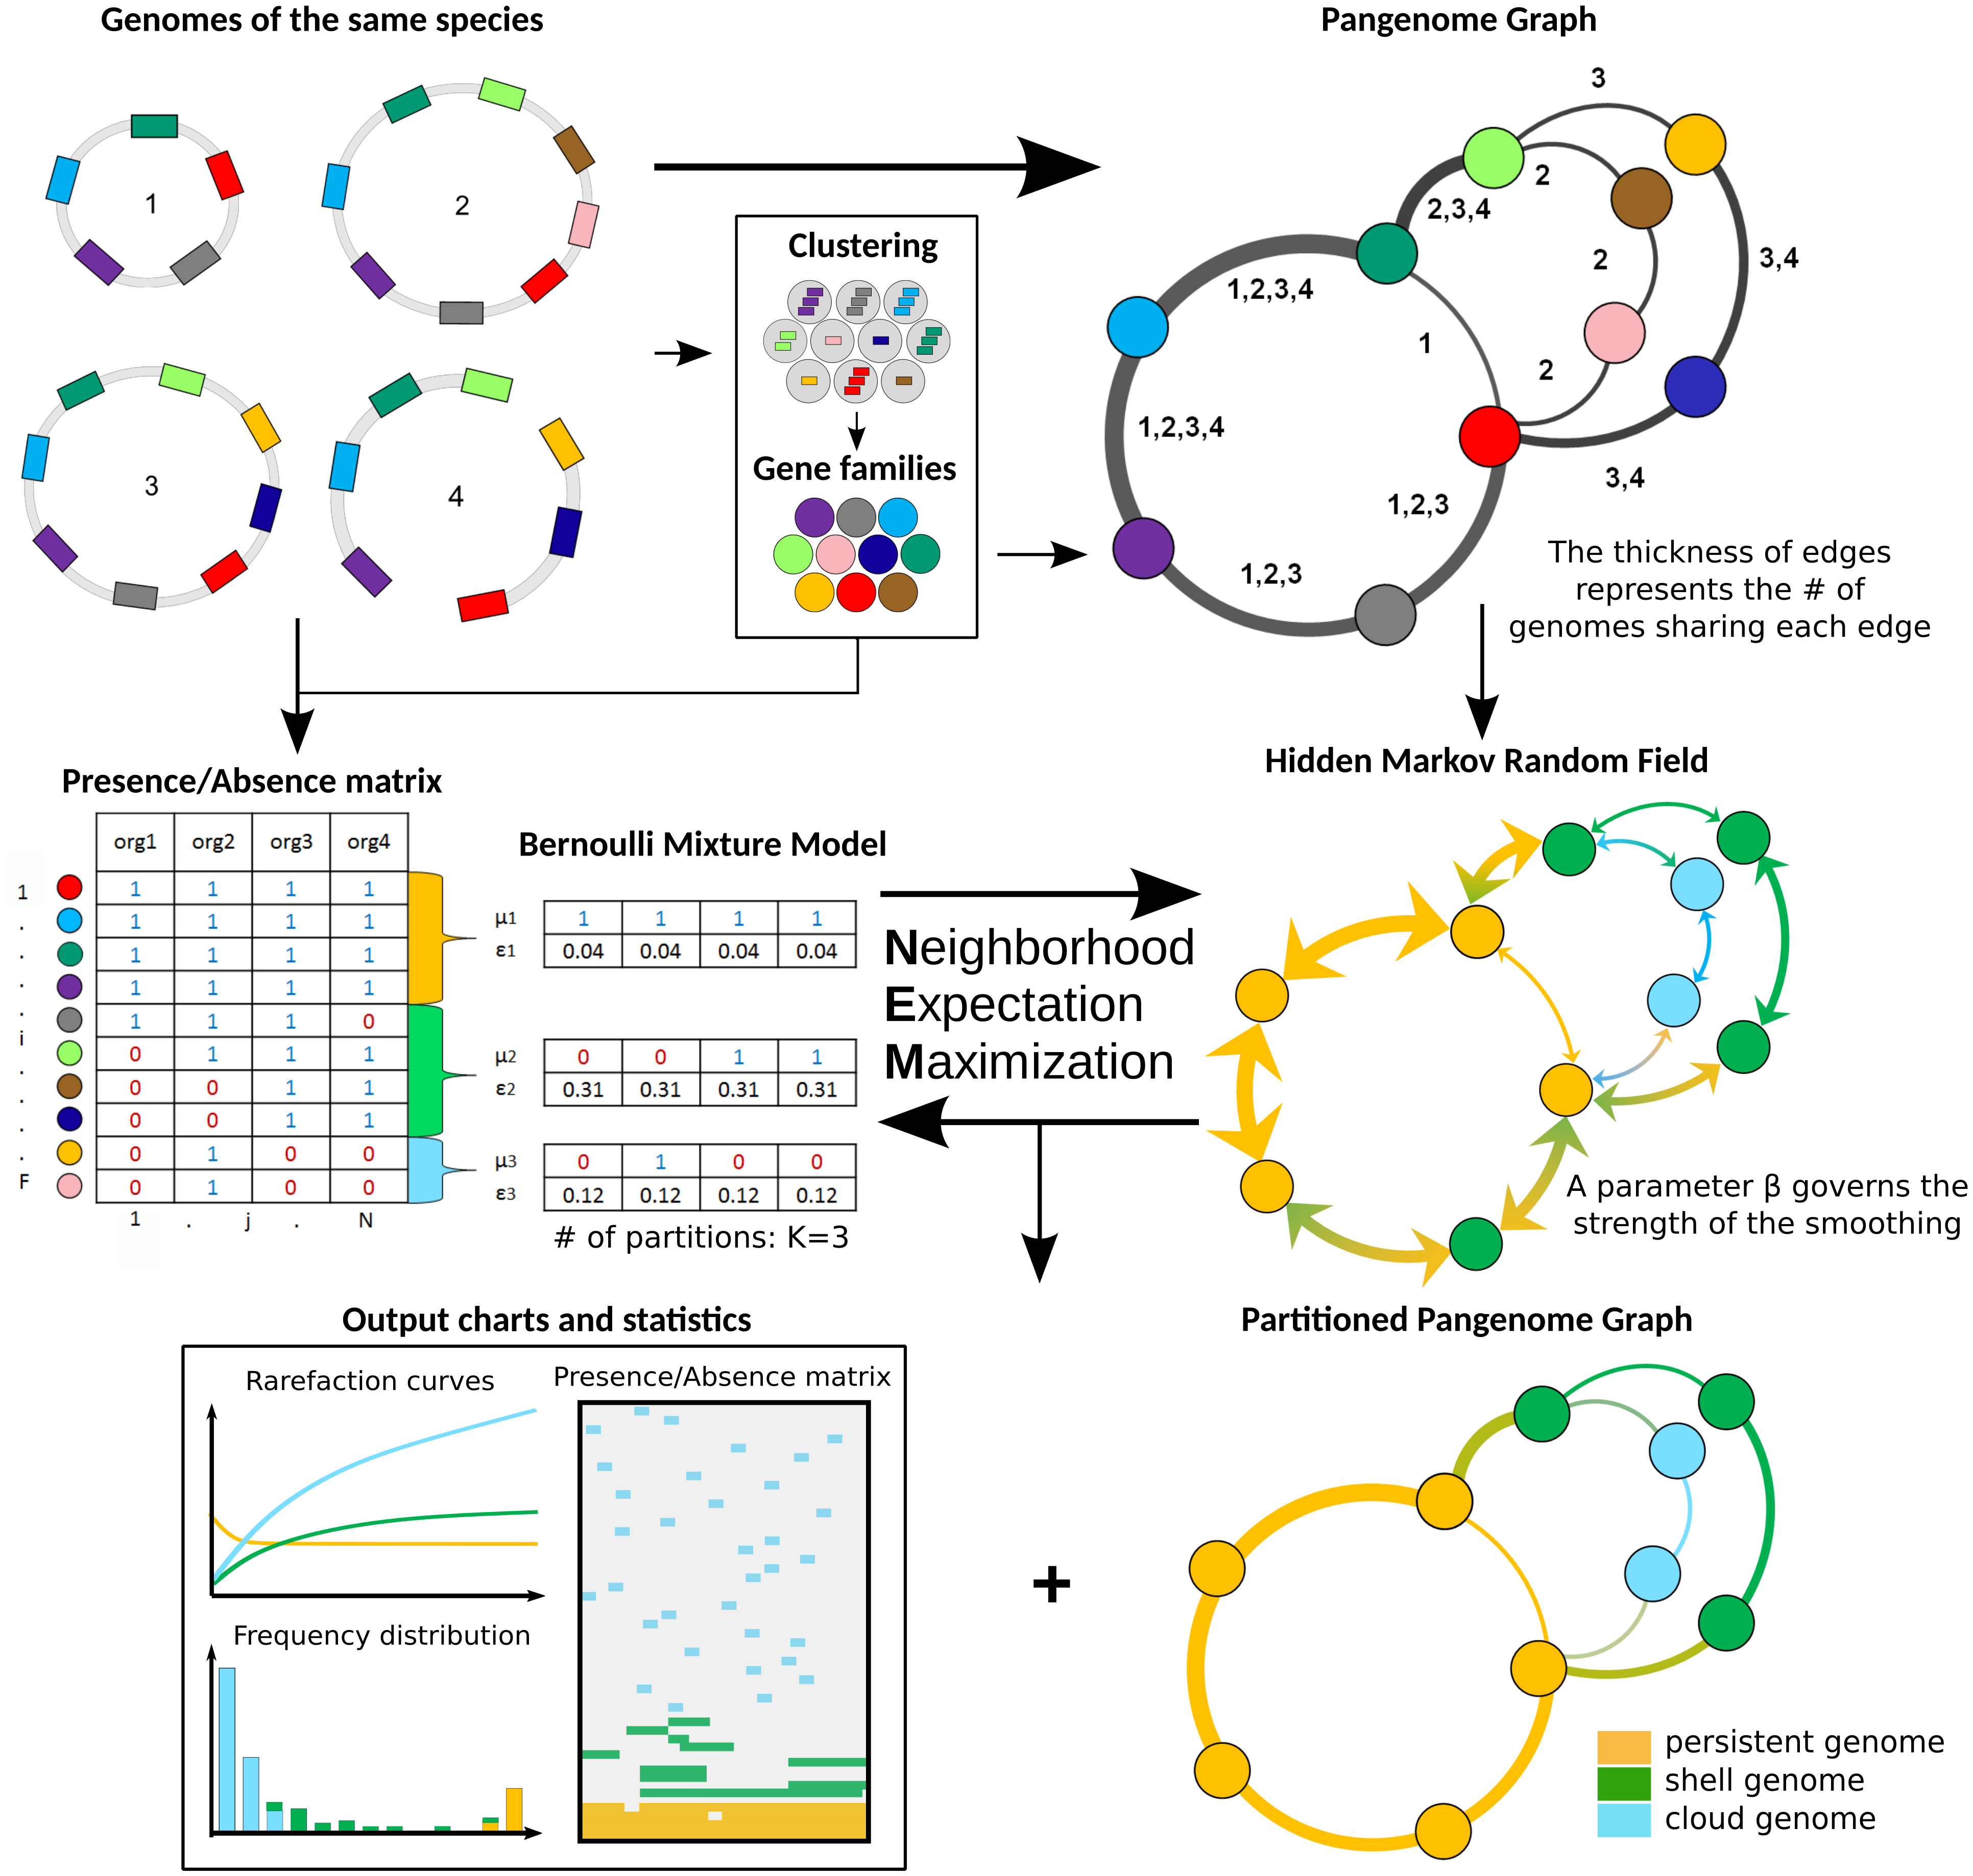
\includegraphics[width=\linewidth]{images/PPanGGOLiN.png}
    \caption[Aperçu général de la méthode PPanGGOLiN]{\textbf{Aperçu général de la méthode PPanGGOLiN.} L'exemple comprend 4 génomes annotés, dont les gènes sont représentés par des rectangles de couleurs. Une même couleur indique que les gènes sont homologues. Les gènes sont clusterisés en familles représentées par des cercles de couleur correspondant aux gènes qu'elles contiennent. Dans le graphe, elles constituent les n\oe uds et sont reliées par des arêtes représentant leur relation de voisinage dans les génomes. Le poids des arêtes représente le nombre de génomes où le voisinage existe. Parallèlement, les familles de gènes sont codées sous la forme d'une matrice de présence/absence qui indique pour chaque famille si elle est présente ou non dans les génomes. Le pangénome est ensuite divisé en K partitions (K = 3 dans cet exemple) en estimant les meilleurs paramètres de partitionnement par un algorithme statistique. PPanGGOLiN renvoie un graphe du pangénome partitionné où les partitions sont superposées au graphe de voisinage. En outre, de nombreux tableaux, graphiques et statistiques sont fournis par le logiciel. Extrait de \cite{gautreau_conceptualisation_2020}}
    \label{fig:ppanggolin}
\end{figure}

Le logiciel PPanGGOLiN intègre une ligne de commande correspondant à chacune de ces étapes, et un workflow pour construire et partitionner automatiquement le pangénome à partir des fichiers de génome. Le pangénome est enregistré dans un fichier au format HDF5 assurant une compréhension et une structuration des données efficaces. Une fois le graphe de pangénome obtenu, plusieurs commandes permettent de réaliser des analyses automatiques, avec des rapports sous forme de tableaux ou de figures.

\newpage
\subsection{Construction du graphe de pangénome}

PPanGGOLiN utilise comme données d'entrée un jeu de génomes procaryotes de la même espèce\footnote{Cette description correspond à l'utilisation prévue par PPanGGOLiN. Néanmoins, PPanGGOLiN a déjà été utilisé avec des génomes appartenant à une même Famille ou encore sur des familles de phages \cite{pfeifer_bacteria_2021}}. Ces génomes peuvent déjà être annotés et donc contenir les gènes (format GFF ou GBFF) ou alors contenir uniquement la séquence nucléique. Dans le second cas, PPanGGOLiN prédira les gènes en utilisant la méthode Prodigal \cite{hyatt_prodigal_2010}. Il détecte également les ARNs à l'aide des logiciels ARAGORN et Infernal \cite{laslett_aragorn_2004,nawrocki_infernal_2013}. 

PPanGGOLiN est un outil reposant sur les familles de gènes pour la construction du pangénome. Il regroupe les gènes en familles en utilisant l’outil MMSeqs2 \cite{steinegger_mmseqs2_2017}, qui applique un workflow automatique de clustering. Ce processus permet de regrouper les gènes homologues en familles avec un seuil de 80 \% d’identité et 80 \% de couverture sur les deux séquences, en s’appuyant sur l’algorithme de clustering \textit{Connected Component}. Bien que cette méthode soit efficace, elle présente une limite dans la gestion des fragments de gènes. Pour y remédier, une étape de défragmentation est intégrée afin de réassigner ces fragments à leurs familles d’origine. Cette correction repose sur un réalignement des séquences représentantes de chaque famille avec MMSeqs2, en conservant les mêmes paramètres d’identité et de couverture, mais en adaptant la couverture à la plus petite des deux séquences comparées. Enfin, un algorithme de clustering, prenant en compte la taille des familles et des séquences, est appliqué pour regrouper les fragments avec leur séquence complète correspondante.

Le graphe de pangénome est ensuite construit à partir des familles (n\oe uds du graphe) et de leur relation de voisinage dans les génomes (arêtes). Deux n\oe uds sont connectés si les familles de gènes correspondantes contiennent au moins une paire de gènes adjacents dans un génome. Les arêtes sont étiquetées avec les identifiants des génomes correspondants et pondérées par la proportion de génomes partageant ce lien.

\subsection{Partitionnement du graphe}

Pour partitionner le graphe, PPanGGOLiN commence par classer les familles de gènes en K partitions ($K\geq2$) à partir d’une matrice binaire indiquant la présence (1) ou l’absence (0) d’un gène dans un génome donné. Le partitionnement s’appuie sur un modèle de mélange de Bernoulli (BMM) estimé via l’algorithme d’Expectation-Maximization (EM), appelé BinEM. En plus des catégories \textit{persistent} et \textit{cloud}, $K-2$  partitions définissent le génome \textit{shell}\footnote{Le nombre de partitions K peut être fixé par l’utilisateur, sinon il est déterminé automatiquement}.

Dans ce modèle, chaque famille de gènes suit une distribution de mélange où les proportions d’appartenance aux partitions sont estimées. Pour éviter le sur-ajustement, une contrainte initiale impose une dispersion homogène au sein d’une même partition.
Chaque famille de gènes est affectée à une partition unique en fonction de sa probabilité d’appartenance, assignée automatiquement si cette probabilité dépasse 0,5 ; sinon, elle est placée dans la partition de fréquence intermédiaire (si K=3, cette partition correspond au \textit{shell}). Pour choisir K, le modèle exécute plusieurs partitionnements et calcule le critère ICL (\textit{Integrated Completed Likelihood})\footnote{ Le critère ICL correspond à un critère BIC (\textit{Bayesian Information Criterion}). Le BIC estime la vraissemblance du modèle à partir du nombre d'observations dans l'échantillon et du nombre de paramètres libres du modèle. L'ICL ajoute une penalité basé sur l'entropie moyenne estimé.}, qui équilibre la qualité du modèle et la complexité, permettant ainsi de sélectionner la valeur optimale de K.

A partir du graphe de pangénome, l’algorithme de \textit{machine learning} \textbf{NEM} (Neighboring Expectation - Maximization) \cite{soares_clustering_1997} améliore le partitionnement en intégrant les informations de contiguïté dans les génomes via un champ de Markov caché, favorisant le regroupement de gènes voisins dans la même partition. Ce modèle lisse la classification en prenant en compte la structure du graphe, bien que la détermination du nombre optimal de partitions K repose d’abord sur BinEM.

Enfin, le partitionnement obtenu est reporté sur le graphe de pangénome. Ce graphe partitionné peut être visualisé et exploré via un fichier de sortie, généré par PPanGGOLiN et visualisable dans l'outil Gephi \cite{bastian_gephi_2009}. Un exemple de graphe partitionné, correspondant au pangénome de \textit{Acinetobacter Baumannii}, est présenté sur la \autoref{fig:pangenomeBaumannii}. Sur le graphe, on peut voir de longs chemins de familles persistantes (orange), entrecoupés de portions de familles variables \textit{shell} (vert) ou \textit{cloud} (bleu). L'exploration et l'analyse de ces régions variables (encadré de la \autoref{fig:pangenomeBaumannii}, par exemple) est particulièrement intéressante, puisque c'est dans ces zones que l'on va retrouver les régions de plasticité génomique.

\begin{figure}[htbp]
    \centering
    \includegraphics[width=0.6\linewidth]{images/pangenomeAcioneto.png}
    \caption[Graphe de pangénome de \textit{Acinetobacter baumannii}]{\textbf{Graphe de pangénome de \textit{Acinetobacter baumannii}.} Le pangénome est construit avec PPanGGOLiN à partir de 3117 génomes de \textit{A. baumannii}. Les arêtes reliant les familles \textit{persistent}, \textit{shell} et \textit{cloud} sont respectivement colorées en orange, vert et bleu. Les connexions entre familles de gènes appartenant à différentes partitions sont représentées par des couleurs mélangées. Pour améliorer la lisibilité, les familles comptant moins de 20 gènes ne sont pas affichées, bien qu'elles représentent 84,68 \% des n\oe uds (principalement des familles à un seul gène). Un encadré dans le coin supérieur gauche zoome sur une région ramifiée où plusieurs chemins alternatifs \textit{shell} et \textit{cloud} sont présents dans l'espèce. Cette région est impliquée dans la biosynthèse du principal antigène polysaccharidique de \textit{A. baumannii}. Les deux chemins les plus fréquents (Sv12/PSgc12 et Sv9/PSgc9) sont mis en avant en kaki et vert fluorescent.}
    \label{fig:pangenomeBaumannii}
\end{figure}

\section{La méthode PanRGP}

Le logiciel PPanGGOLiN intègre une méthode pour l'identification des régions de plasticité génomique et la prédiction des spots d'insertion, la méthode panRGP \cite{bazin_panrgp_2020}. Cette méthode repose sur l'utilisation du graphe de pangénome partitionné pour ne pas avoir à comparer l'ensemble des génomes (ce qui est déjà fait dans la construction du pangénome) et donc d'être plus efficace que les outils de génomique classique.

\subsection{Identification des régions de plasticité génomique}

Les régions de plasticité génomique sont des objets génomiques : la méthode de prédiction décrite dans la \autoref{fig:panRGP} est appliquée à chaque génome du pangénome, sur lesquels on a projeté les partitions du pangénome.

Pour chaque gène du génome, on calcule un score $s_g$ de manière séquentielle le long des contigs qui est égal au score du gène précédent auquel on applique une pénalité ou une prime en fonction de la partition du gène. Si le gène est \textit{shell} ou \textit{cloud}, on applique une prime correspondant à la somme de 2 constantes, $v$ qui favorise le gène variable et $\epsilon$ pour égaliser les résultats quelque soit le sens de lecture du contig. Si le gène est \textit{persistent}, on applique une pénalité $p$. Pour pénaliser la succession de gènes \textit{persistent}, la pénalité est exponentiellement proportionnelle au nombre ($n$) de gènes \textit{persistent} successifs précédents ($p^n$).   

Si le génome est linéaire, le premier gène de chaque contig aura un score de 0. Dans le cas des séquences circulaires, un premier gène est choisi et un score initial de 0 lui est attribué, puis l’algorithme assigne un score à tous les autres gènes. À la fin du contig, le gène avec un score de 0 est réévalué. Ce nouveau score sert de base pour exécuter une nouvelle boucle de calcul de score qui s'arrête dès qu'un gène obtient un score de 0 ou jusqu’à atteindre le dernier gène du contig.

\begin{figure}[htbp]
    \centering
    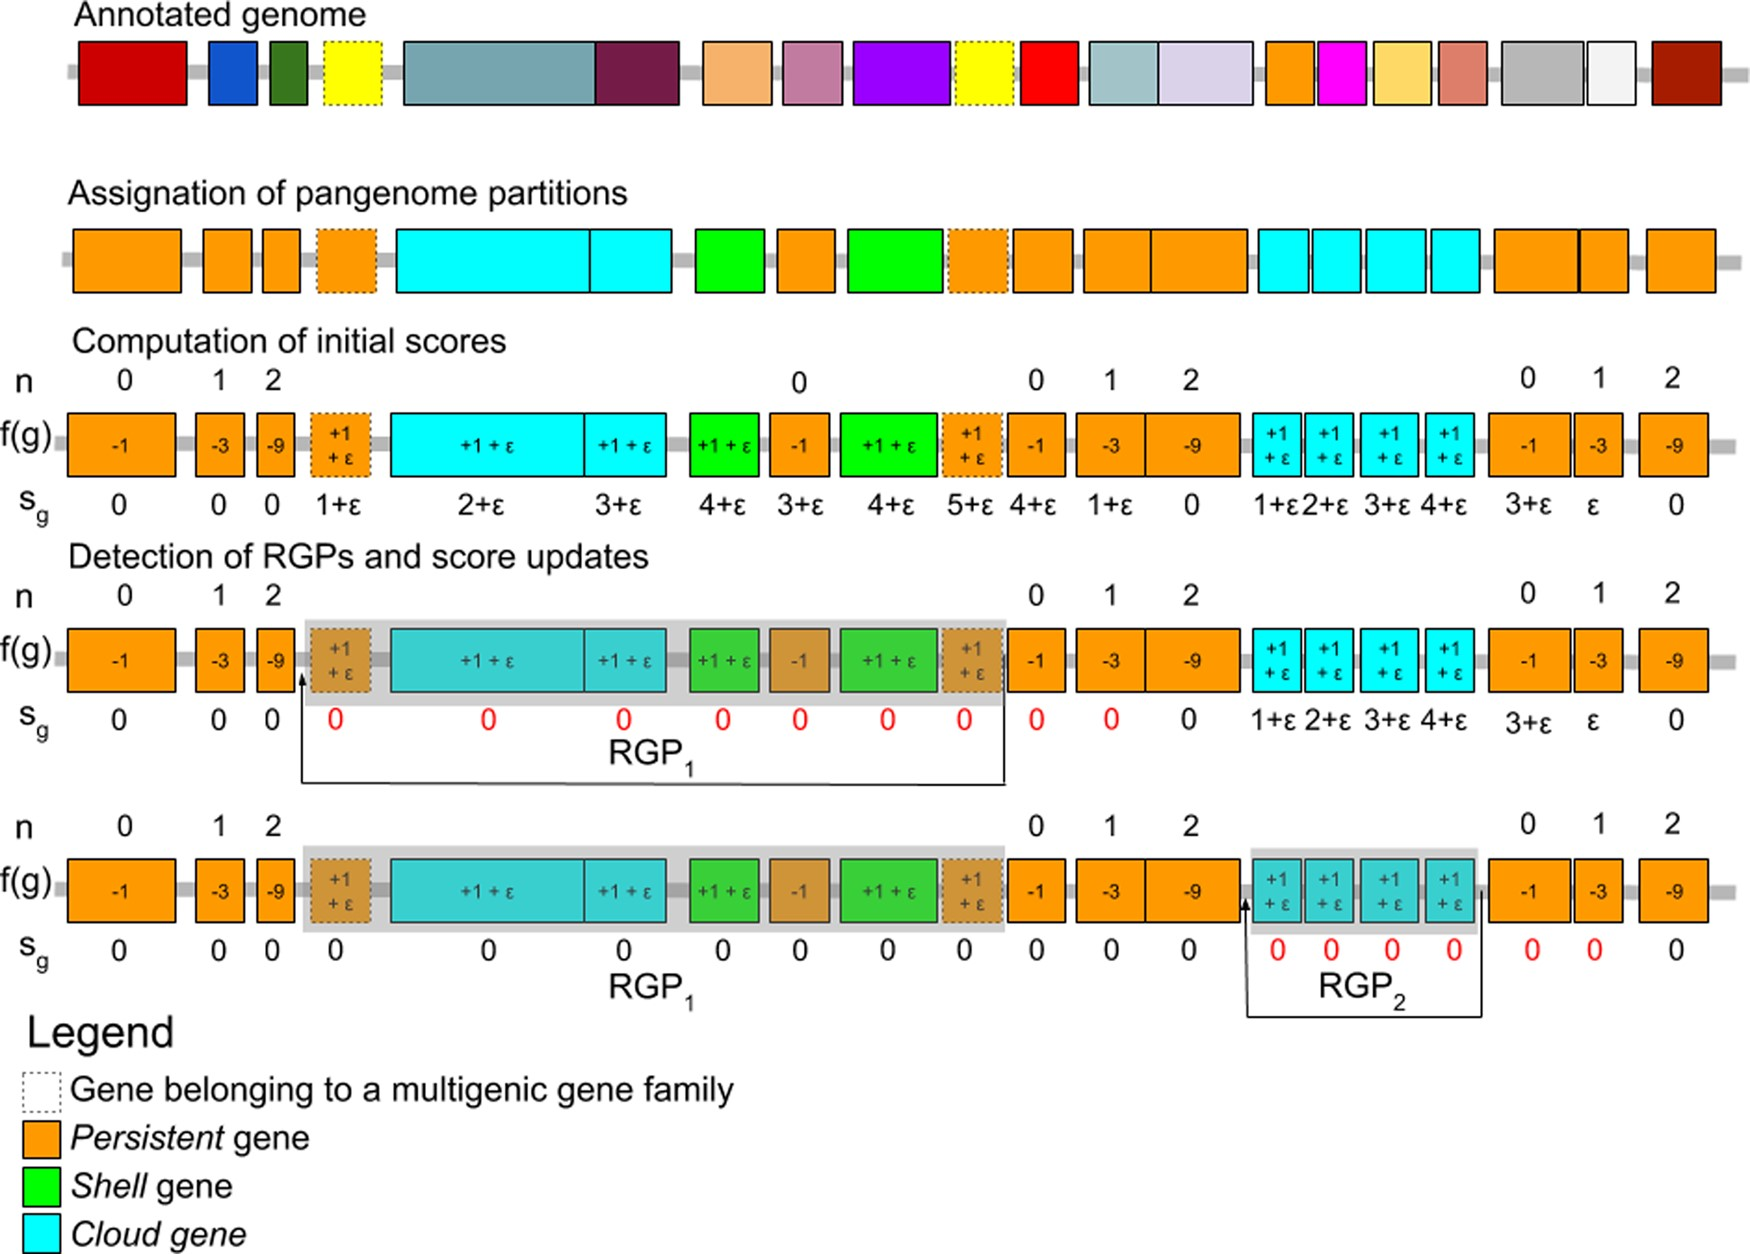
\includegraphics[width=0.8\linewidth]{images/panRGP.jpeg}
    \caption[PanRGP : vue d’ensemble de la méthode de détection des RGP]{\textbf{PanRGP : vue d’ensemble de la méthode de détection des RGP.} Les boîtes représentent les gènes codant des protéines : les couleurs orange, vert et bleu correspondent respectivement aux partitions \textit{persistent}, \textit{shell} et \textit{cloud}. Les boîtes en pointillés signalent les gènes appartenant à des familles multigéniques. Dans cet exemple, deux RGP sont détectées : RGP1 avec un score de 5 et RGP2 avec un score de 4. La valeur n associée à chaque gène correspond au nombre de gènes persistants consécutifs en aval. Les valeurs $f(g)$ représentent le résultat d'une fonction utilisée pour calculer le score de chaque gène ($s_g$). Ici, les paramètres par défaut p et v sont fixés respectivement à 3 et 1.}
    \label{fig:panRGP}
\end{figure}

Pour détecter les RGPs, l’algorithme parcourt chaque contig à la recherche du gène ayant le score le plus élevé, à condition qu’il dépasse le seuil $s_{min}$ (fixé par défaut à 4). Ce gène marque la fin initiale de la RGP. Ensuite, les gènes situés en amont sont ajoutés progressivement jusqu’à rencontrer un gène dont le score est nul. La région est alors considérée comme une RGP uniquement si elle contient un nombre de nucléotide supérieur au seuil minimal attendu $l_{min}$ (fixé par défaut à 3 000 bp). Enfin, le score de la RGP est recalculé en repartant du dernier gène détecté, en appliquant la même méthode de calcul que précédemment.

\subsection{Prédiction des spots d'insertion}

Les spots correspondent à des régions où de nombreux éléments se sont insérés au cours de l'évolution, et donc ce sont des régions fortement variables. Aux extrémités de chaque RGP, on sélectionne un nombre \textit{c} de gènes persistants non multigéniques, convertis en familles de gènes pour rendre l’algorithme indépendant de l’orientation.

\newpage

Un graphe $G(V, E)$ est construit, où chaque n\oe ud représente les bordures d’une RGP et chaque arête relie deux n\oe uds ayant des ensembles de familles de gènes similaires. Deux bords sont considérés comme proches si leurs \textit{e} premières familles sont identiques ou si leurs ensembles ordonnés se chevauchent d’au moins \textit{o} familles. Lorsque tous les bords de deux RGPs correspondent, une arête est ajoutée, et les composantes connexes du graphe définissent les spots, auxquels sont associées les RGPs correspondantes.

Les paramètres par défaut sont $c=3$, $e=1$, $o=2$. Chaque spot est évalué selon plusieurs métriques, comme le nombre de RGPs et de familles de gènes. Les RGPs sans $c$ gènes persistants consécutifs ne sont pas prises en compte, car elles sont soit incomplètes (bords de contigs), soit correspondent à des plasmides.

\section{La méthode PanModule}

Dans les génomes, et notamment dans les GIs et les spots, des groupes de gènes sont supposés avoir suivi la même histoire évolutive. Ces ensembles de gènes, cooccurrents et colocalisés, sont appelés des \textbf{modules conservés}. La méthode panModule \cite{bazin_panmodule_2021}, intégrée à PPanGGOLiN, permet de détecter ces modules depuis le graphe de pangénome partitionné. 

\newpage

Tout d'abord, un pangénome est reconstruit à partir des génomes, mais celui-ci intègre, en plus des arêtes de voisinage directes, des arêtes entre les familles séparées dans les génomes d'un espace intergénique inférieur à $t$ gènes. Lorsque $t > 1$, cela équivaut à appliquer une \textbf{fermeture transitive} partielle sur les graphes de génomes, ce qui permet de relier des familles même si leurs gènes ne sont pas directement adjacents. Cette approche est particulièrement utile lorsqu’un module génomique est interrompu par l’insertion d’un gène (comme une séquence d’insertion) ou lorsque des gènes ont été perdus à la suite d’un événement de délétion ou de pseudogénisation.

Les arêtes vont ensuite être filtrées selon deux \textbf{coefficients de similarité de Jaccard} :

\begin{equation}
J(v_i, e_{i,j}) = \frac{w_{e_{i,j}}}{w_{v_i}}, \quad J(v_j, e_{i,j}) = \frac{w_{e_{i,j}}}{w_{v_j}}
\label{eq:jaccard}
\end{equation}

où :
\begin{itemize}
    \item $w_{v_i}$ et $w_{v_j}$ correspondent au nombre de gènes associés aux familles $v_i$ et $v_j$, respectivement.
    \item $w_{e_{i,j}}$ représente le nombre de paires de gènes ayant servi à créer l’arête $e_{i,j}$ entre les nœuds $v_i$ et $v_j$.
\end{itemize}

Un seuil $s$ est défini comme la similarité minimale de Jaccard nécessaire pour considérer une arête comme appartenant à un module. Si les deux coefficients de Jaccard vérifient :

\begin{equation}
J(v_i, e_{i,j}) > s \quad \text{et} \quad J(v_j, e_{i,j}) > s
\end{equation}

alors l’arête est conservée ; sinon, elle est supprimée du graphe. De plus, les n\oe uds correspondant à des familles de gènes présentes dans moins de $m$ génomes sont également retirés.

Après cette phase de filtrage, les \textbf{composantes connexes} du graphe sont extraites à l’aide d’un algorithme de \textbf{parcours en largeur (BFS)} modifié. Une composante est considérée comme un \textbf{module prédit} si elle contient au moins trois n\oe uds appartenant aux familles \textit{shell}, \textit{cloud} ou multigéniques persistantes, selon la classification PPanGGOLiN. En revanche, les modules constitués de \textbf{familles persistantes non multigéniques} ne sont pas pris en compte. Ces familles correspondent généralement à des régions synténiques conservées dans la majorité des génomes étudiés, avec peu ou pas d’événements de réarrangement.

Les modules prédits peuvent ensuite être associés aux autres analyses de PPanGGOLiN, en identifiant sur quelles RGPs et dans quels spots sont retrouvés les modules.